\documentclass[a4paper]{article}
\usepackage{forest}
\usepackage{float}
\usepackage{geometry}
\usepackage{caption, subcaption}
\usepackage{listings}
\usepackage{hyperref}
\usepackage{graphicx}
\usepackage{ragged2e}
\usepackage{color}
\usepackage{xepersian}
\usepackage{subfiles}
\newgeometry{left=1.4cm, right=1.4cm, bottom=2.0cm, top=2.0cm}
\settextfont[Scale=1]{XB Roya}
\renewcommand{\baselinestretch}{1.5}
\definecolor{dkgreen}{rgb}{0,0.6,0}
\definecolor{gray}{rgb}{0.5,0.5,0.5}
\definecolor{mauve}{rgb}{0.58,0,0.82}
\definecolor{commentColor}{rgb}{0.6,0.6,0.60}

\title{گزارش پروژه ارزیابی عملکرد پروتکل مسیریابی اطلاعاتی \\ \lr{RIP: Routing
Information Protocol} \\ \small{\lr{A Routing Protocol Based on the
Distance-Vector Algorithm}}}
\author{علیرضا سلطانی نشان \\ \small{استاد راهنما: آقای دکتر مهدی امینیان}}

\begin{document}
\maketitle
\tableofcontents
\listoffigures

\section{هدف کلی این آزمایش}

هدف از انجام این آزمایش آشنایی با روش پیکربندی و آنالیز عملکرد مدل پروتکل
اطلاعات مسیریابی یا \lr{RIP} می‌باشد.

\section{بررسی اجمالی}

یک مسیریاب بایستی قادر باشد که با نگاه کردن به آدرس مقصد یک بسته، بهترین مسیر را
برای ارسال بسته با آدرسی مشخص انتخاب کند. مسیریاب این کار را با مشورت با جدول
\lr{Forwarding} انجام می‌دهد. مسئله پایه‌ای مسیریاب آن است که مسیریاب‌ها چگونه
اطلاعات جداول ارسال خود را بدست می‌آورند؟

الگوریتم‌های مسیریابی نیازمند ساخت جداول مسیریابی و آدرس‌دهی هستند. مسئله ساده
مسیریاب‌ها پیدا کردن کم‌هزینه‌ترین مسیر بین هر دو گره است به گونه‌ای که هزینه یک
مسیر برابر با مجموع هزینه‌های تمام لبه‌ها باشد که باعث ساخت یک مسیر
می‌شوند.مسیریابی در شبکه‌ها با استفاده از پروتکل‌هایی مانند RIP انجام می‌شود که
به صورت توزیع‌شده و دینامیک مسیرهایی با کمترین هزینه را پیدا می‌کنند. این
پروتکل‌ها با تغییرات در هزینه لینک‌ها یا خرابی گره‌ها و لینک‌ها سازگار هستند. 

\subsection{الگوریتم \lr{Distance vector}}

یکی از الگوریتم‌های اصلی مسیریابی، الگوریتم \lr{Distance-Vector} است. در این
الگوریتم هر گره یک بردار شامل هزینه‌ها را به سایر گره‌ها می‌سازد. این بردار به
همسایگان مستقیم ارسال می‌شود. پروتکل \lr{RIP} نمونه‌ای از این الگوریتم است که به
صورت دوره‌ای هر ۳۰ ثانیه اطلاعات مسیریابی را منتشر \lr{Advertissment} می‌کند  و
در صورت وقوع تغییر \lr{Trigger} به روزرسانی‌های فوری ارسال می‌شوند.

\subsection{آنالیز عملکرد مسیر‌های ساخته شده}

با استفاده از پروتکل \lr{ICMP} می‌توان با \lr{Ping} گرفتن و ارسال بسته‌های
\lr{Async} به مسیر‌های مقصد، عملکرد مسیر‌های ایجاد شده را بررسی کرد.

\subsection{اهداف این آزمایش در شبیه‌ساز \lr{Opnet}}

در این آزمایش، شبکه‌ای با استفاده از پروتکل \lr{RIP} تنظیم کرده‌ایم که جداول 
مسیریابی را در مسیریاب ایجاد می‌کند و می‌توانیم آن‌ها بررسی کنیم. همچنین
می‌توانیم با انجام سناریو \texttt{Failure} تاثیر لینک خرابی لینک‌ها را در پرتکل
\lr{RIP} مشاهده کنیم.

\section{تمرینات}

لازم به ذکر است که تمام تمارین انجام شده در نرم‌افزار شبیه‌سازی شبکه \lr{Opnet}
انجام شده است.

\begin{enumerate}
    \item با گراف‌هایی که از ارسال ترافیک در \lr{RIP} بدست آمده است، ترافیک بین
    سناریو‌های \texttt{Failure} و \texttt{No\_Failure} را با هم مقایسه و بررسی
    کنید (حالت نمایش نمودار را میله‌ای کنید).

    \begin{figure}[h!]
        \centering
        \begin{subfigure}{0.45\textwidth}
            \centering
            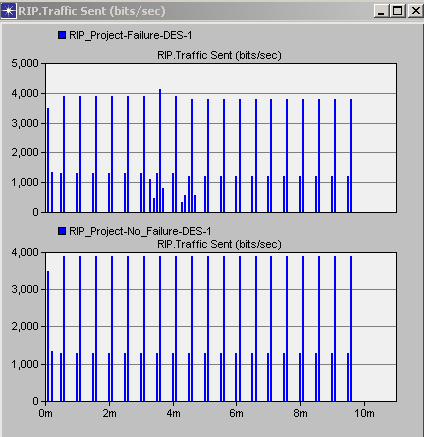
\includegraphics[width=\textwidth]{./figs/traffic_sent.png}
            \caption{شبیه‌سازی ترافیک ارسالی در دو سناریو}
        \end{subfigure}
        \hfill
        \begin{subfigure}{0.45\textwidth}
            \centering
            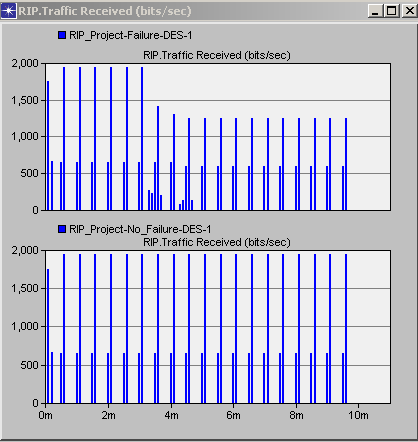
\includegraphics[width=\textwidth]{./figs/traffic_received.png}
            \caption{شبیه‌سازی ترافیک دریافتی در دو سناریو}
        \end{subfigure}
        \caption{ترافیک‌های شبیه‌سازی شده در \lr{RIP}}
    \end{figure}

    ترافیک‌های ارسال در دو سناریو \lr{Failure} و \lr{No\_Failure} رفتار کاملاً
    متفاوتی با توجه به ماهیت \lr{RIP} دارند.
    
    ترافیک ارسال‌شده در سناریو \lr{Failure} در لحظات مشخصی اوج می‌گیرد که این
    افزایش ترافیک احتمالاً به دلیل تلاش‌های \lr{RIP} برای بازیابی یا به روزرسانی
    جدول‌های مسیریابی بعد از وقوع خرابی در شبکه می‌باشد. نرخ ارسال معمولاً به
    $4.5K$ بیت بر ثانیه در پیک‌های ترافیک مشاهده می‌شود. حجم ترافیک ارسال به
    دلیل مکانیزم‌های باز‌ارسال اطلاعات توسط \lr{RIP} زیاد است تا درنهایت بتواند
    در مسیری مناسب اطلاعات را منتشر و ارسال کند. این رفتار با توجه به ماهیت
    \lr{RIP} ناهنجاری نیست و کاملاً طبیعی می‌باشد.

    در سناریو \lr{No\_Failure} مشخص است که نرخ ترافیک ارسال‌شده کمتر از سناریو
    \lr{Failure} است و به صورت پایدار در $4K$ بیت بر ثانیه باقی می‌ماند. این
    نمودار‌ها نشان می‌دهند که در حالت بدون خرابی، پروتکل \lr{RIP} به صورت
    دوره‌ای اطلاعات مسیریابی را ارسال می‌کند وکه نیازی به ارسال‌های مکرر یا
    اضافی برای ریکاور کردن اطلاعات ندارد.
    
    \item تاثیر سناریو \lr{Failure} بین \lr{Router 1} و \lr{Router 2} را بر اساس
    جدول \lr{Router 1} توضیح دهید.

    \begin{figure}[h!]
        \centering
        \begin{subfigure}{0.45\textwidth}
            \centering
            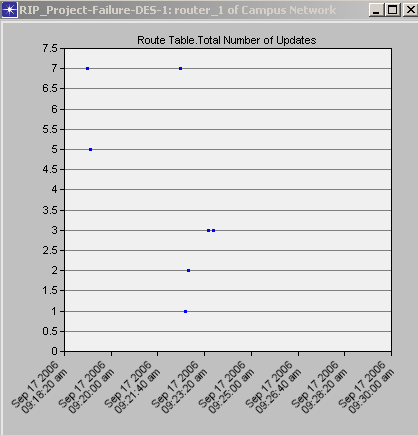
\includegraphics[width=\textwidth]{./figs/router_1_failure_update.png}
            \caption{تعداد به روزرسانی‌های مسیریاب اول}
        \end{subfigure}
        \hfill
        \begin{subfigure}{0.45\textwidth}
            \centering
            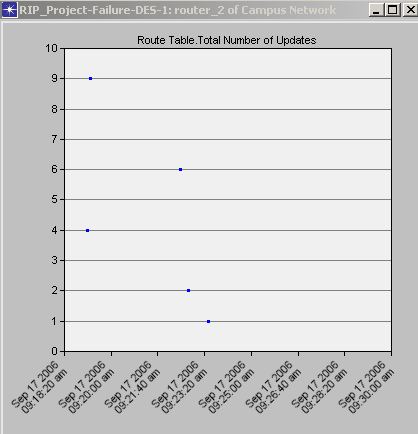
\includegraphics[width=\textwidth]{./figs/router_2_failure_update.png}
            \caption{تعداد به روزرسانی‌های مسیریاب دوم}
        \end{subfigure}
        \caption{به روزرسانی‌های مسیریاب‌ها در هنگام برخورد به خطا}
    \end{figure}

    در مسیریاب اول تعداد به روزرسانی‌های جدول مسیریابی افزایش داشته است که
    نشان‌دهنده تعداد تلاش مسیریاب برای یافتن مسیر جایگزین برای ارسال پکت‌ها
    می‌باشد.

    اگر به تغییرات دو جدول در تعداد به روزرسانی‌ها دقت کنیم می‌توان متوجه شد
    که مسیریاب اول بعد از قطع ارتباط (مشکل در ارتباط) جدول مسیریابی خود را
    بازسازی می‌کند و اطلاعات مربوط به مسیر‌های دیگر را دریافت می‌کند (پدیده
    \lr{Retry}).

    افزایش به روزرسانی‌های مسیریاب اول نسبت به مسیریاب دوم بیشتر بوده است پس
    می‌توان نتیجه گرفت که مسیریاب اول مستقیماً تحت تاثیر قطع لینک ارتباطی
    قرار داشته است که بعد از مدتی تعداد به روزرسانی‌ها به مقدار ثابتی کاهش
    یافته است که یعنی مسیریاب اول به مسیر جدیدی دست یافته است و می‌تواند از
    طریق آن ارسال پکت‌ها را انجام دهد و به حالت پایدار رسیده است.

    \item سناریو دیگری به نام \texttt{Q3\_Recover} بسازید. در این سناریو لینک
    ارتباطی باید بین \lr{Router\_1} و \lr{Router\_2} باشد به گونه‌ای که بعد از
    ۴۰۰ ثانیه ریکاور شود. شبیه‌سازی این سناریو را انجام دهید و با استفاده از
    نمودار بدست آمده نمودار \lr{Total Number of Updates} مسیریاب اول را با
    نمودار‌های \texttt{No\_Failure} و \texttt{Failure} بررسی و آنالیز کنید.

    \begin{figure}[h!]
        \centering
        \begin{subfigure}{0.45\textwidth}
            \centering
            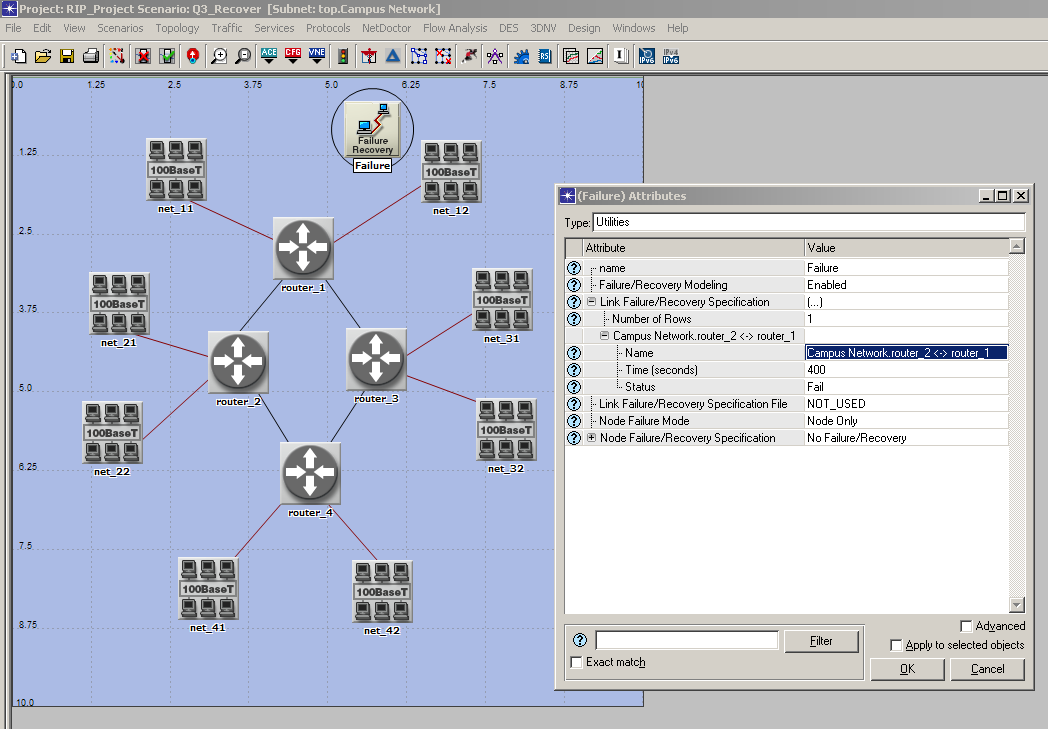
\includegraphics[width=\textwidth]{./figs/q3_recover_cfg.png}
            \caption{تعداد به روزرسانی‌های مسیریاب اول}
        \end{subfigure}
        \hfill
        \begin{subfigure}{0.45\textwidth}
            \centering
            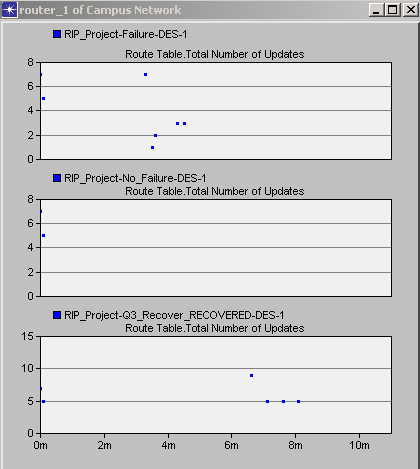
\includegraphics[width=\textwidth]{./figs/comparison_q3_nf_f.png}
            \caption{تعداد به روزرسانی‌های مسیریاب دوم}
        \end{subfigure}
        \caption{به روزرسانی‌های مسیریاب‌ها در هنگام برخورد به خطا}
    \end{figure}

    \begin{enumerate}
        \item سناریوی \texttt{Failure} (قطع لینک):
        در نمودار اول، قطع لینک در ۲۰۰ ثانیه باعث افزایش تعداد به‌روزرسانی‌ها
        می‌شود، زیرا \texttt{Router\_1} سعی می‌کند مسیری جایگزین پیدا کند. این
        وضعیت ناپایدار تا زمانی که شبکه به یک حالت جدید برسد ادامه دارد.
        \item سناریوی \texttt{No\_Failure} (بدون خطا): نمودار دوم نشان می‌دهد که
        جدول مسیریابی \texttt{Router\_1} بدون قطع لینک کاملاً پایدار است.
        به‌روزرسانی‌های جدول مسیریابی تقریباً صفر باقی مانده است.
        \item سناریوی \texttt{Q3\_Recover} (بازیابی لینک):
        در نمودار سوم، قطع لینک در ۲۰۰ ثانیه باعث افزایش تعداد به‌روزرسانی‌ها
        می‌شود، مشابه سناریوی \texttt{Failure}. اما پس از ۴۰۰ ثانیه، زمانی که
        لینک بازیابی می‌شود، تعداد به‌روزرسانی‌ها دوباره افزایش می‌یابد، زیرا
        \texttt{Router\_1} جدول مسیریابی خود را بازسازی کرده و لینک بازیابی‌شده
        را دوباره در نظر می‌گیرد. این امر نشان‌دهنده بازگشت شبکه به حالت پایدار
        است.
    \end{enumerate}
\end{enumerate}
\end{document}